% Created 2024-02-06 Tue 22:54
% Intended LaTeX compiler: pdflatex
\documentclass[11pt]{article}
\usepackage[utf8]{inputenc}
\usepackage[T1]{fontenc}
\usepackage{graphicx}
\usepackage{longtable}
\usepackage{wrapfig}
\usepackage{rotating}
\usepackage[normalem]{ulem}
\usepackage{amsmath}
\usepackage{amssymb}
\usepackage{capt-of}
\usepackage{hyperref}
\usepackage[margin=2cm]{geometry}
\author{Ian Grant}
\date{\today}
\title{Spatiotemporal model of flooding-related 311 calls in New York City}
\hypersetup{
 pdfauthor={Ian Grant},
 pdftitle={Spatiotemporal model of flooding-related 311 calls in New York City},
 pdfkeywords={},
 pdfsubject={},
 pdfcreator={Emacs 29.0.92 (Org mode 9.6.6)}, 
 pdflang={English}}
\makeatletter
\newcommand{\citeprocitem}[2]{\hyper@linkstart{cite}{citeproc_bib_item_#1}#2\hyper@linkend}
\makeatother

\usepackage[notquote]{hanging}
\begin{document}

\maketitle

\section{Introduction}
\label{sec:orge386669}
Pluvial flooding is an increasingly disruptive problem in New York City given increased precipitation due to climate change. Understanding where and when flooding takes place is necessary in order to identify vulnerable areas and assess the efficacy of adaptations. However, urban flood modelling (e.g. with hydrology models) and detection (e.g. with synthetic aperture radar) are both hindered by the physical complexity of the urban environment. An alternative approach to detecting and characterizing floods is to use the rich social and administrative datasets that cities are uniquely able to provide. In this project, I propose to develop a statistical model of New York City's dataset of 311 requests for service in order to better understand the spatiotemporal patterns of flooding in the city.

\begin{figure}[htbp]
\centering
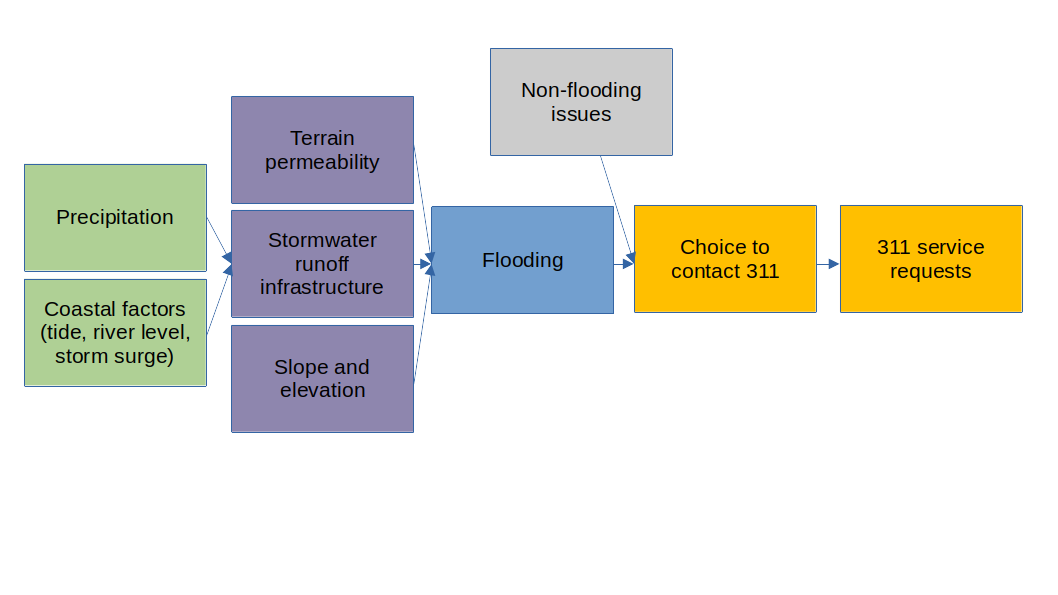
\includegraphics[width=.9\linewidth]{flooding_proposal_conceptual_model.png}
\caption{\label{fig:orgbcdf9af}Conceptual model of flood-related 311 service requests. Meteorological factors (green) are mediated by terrain and infrastructure (purple) to produce flooding (blue). 311 requests are produced by residents' choice to report flooding (orange); some flooding may go unreported, and some requests may not reflect flooding (gray).}
\end{figure}

\section{Statistical approaches}
\label{sec:orgaf7c9d3}
This statistical analysis could take several possible forms, ordered
here by increasing complexity.

\subsection{Spatiotemporal point pattern analysis}
\label{sec:org9c5e740}
The simplest approach would be to treat the 311 requests as a spatiotemporal point pattern. Understanding the degree of spatial and temporal autocorrelation in the dataset would already provide useful information about the scale and duration of the physical processes driving the 311 requests. Similarly, a spatiotemporal clustering approach could be useful for distinguishing flood-driven requests from one-off calls.

\subsection{Spatiotemporal point process model}
\label{sec:org61f6fcb}
An intermediate version of the project could model the calls using a
point process model. Predictor variables could include what we know of
sewer infrastructure, precipitation from MicroNet station or remote
sensing data, and FloodNet sensing data.

\subsection{Statistical analysis of infrastructure improvements}
\label{sec:orgc546f77}
The most complex version of the model could attempt to detect a statistical relationship between the Department of Environmental Protection's (DEP) green infrastructure projects and the local prevalence of 311 requests, controlling for all the factors included in the point process model.

\section{Scope and scale}
\label{sec:org6598624}
A forthcoming analysis by Eric Sanderson (New York Botanical Garden)
suggests that Brooklyn and Queens are the most vulnerable boroughs to
flooding in general. To simply the present project, I will restrict the spatial scope to these boroughs, expanding it to the full city only if the Brooklyn and Queens version is successful. I will attempt to use the full length of the 311 record in the analysis, but I will initially focus on a few notable instances of pluvial flooding as exploratory test cases.

\section{Data}
\label{sec:org8774038}
\subsection{311 requests for service}
\label{sec:org2ef3656}
This dataset goes back to 2010 and contains roughly 35 million requests for service. Each request is geolocated and includes the precise time the request was made. The requests also include descriptions that indicate why the requests were made. An initial query suggests that the dataset includes approximately 150,000 flooding-related requests since 2010.

\subsection{DEM}
\label{sec:org74988d2}
I will use the city's lidar-based DEM to derive relevant features of the terrain, such as slope and elevation.

\subsection{Meteorological data}
\label{sec:org5fe2095}
I will use data from the city's MicroNet system of weather stations for real-time precipitation data. It may also be possible to obtain more fine-grained precipitation data from remote sensing products.

\subsection{Permeability}
\label{sec:org69d3dfb}
In order to measure permeability, I will use the data produced by the DEP's parcel-based study of ground permeability.

\subsection{FloodNet}
\label{sec:orga9582cd}
The city has a relatively new network of ground-based inundation sensors. This would be useful for exploring the statistical relationship between 311 calls and physical inundation. I am discussing access to this data with the project lead at Brooklyn College. 

\subsection{DEP green infrastructure}
\label{sec:orgbdefc04}
I will use the DEP's publicly available database of green
infrastructure projects, some of which are intended to mitigate
flooding.
\end{document}